\begin{frame}
    \frametitle{Motivación: Position control}
    \note{Información extraída de https://youtu.be/pEVsedl2KO4?si=_cwQpRPPUnQ04B3c}
    
    \begin{itemize}
        \item Mover al robot a una ubicación deseada $\state_{des}$
        \item ¿Cómo generar una señal apropiada de control $\controlCommand$?
        \item La localización del robot estimada por medio de un sensor con mediciones $\observation$
    \end{itemize}
    
\end{frame}


\begin{frame}
    \frametitle{Cinemática de un cuerpo rígido}
    \note{Información extraída de https://youtu.be/pEVsedl2KO4?si=_cwQpRPPUnQ04B3c}
    
    \begin{itemize}
        \item Consideremos al robot como un punto de masa
        \item Se mueve libremente en el espacio 1D
    \end{itemize}
    
    
    \begin{center}
        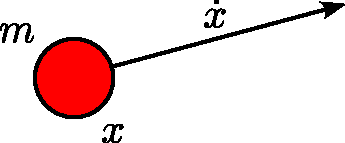
\includegraphics[width=0.4\columnwidth]{images/rigid_body_kinematics.pdf}
    \end{center}
    
\end{frame}

\begin{frame}
    \frametitle{Cinemática de un cuerpo rígido}
    \note{Información extraída de https://youtu.be/pEVsedl2KO4?si=_cwQpRPPUnQ04B3c}
    
    \begin{itemize}
        \item Modelo del sistema: $\state_{t} = \state_{t-1} + \dot{\state} \Delta t$
        \item Estado Inicial: $\state_{0} = 0, \, \dot{\state} = 0$
    \end{itemize}
    
    
    \begin{center}
        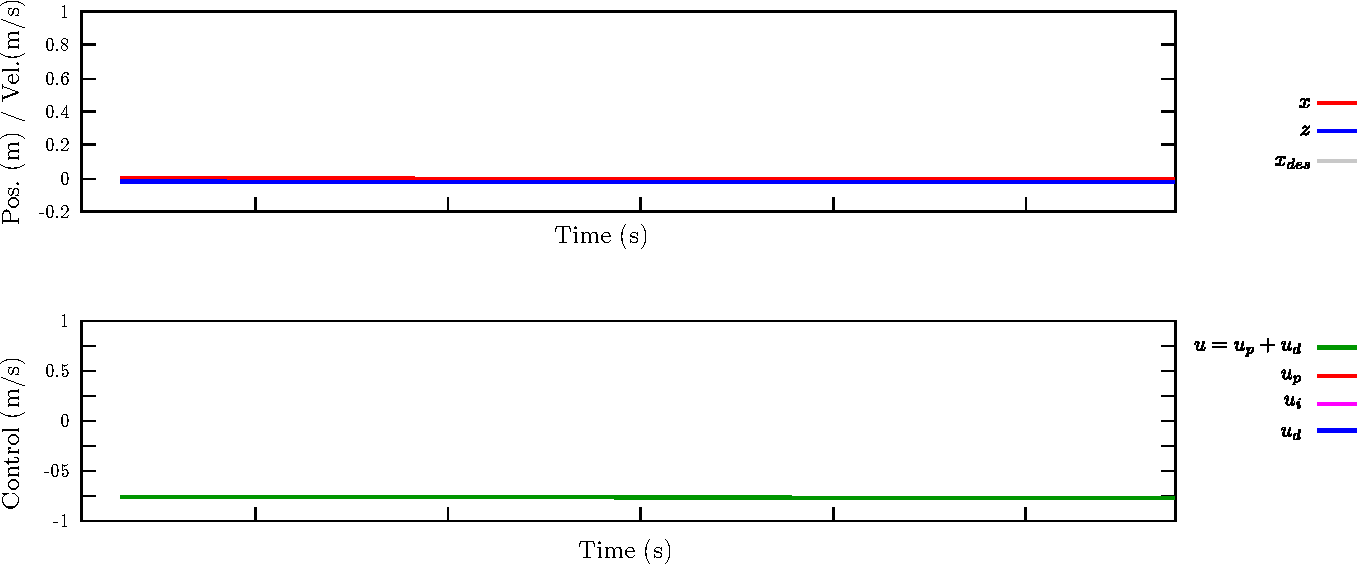
\includegraphics[width=0.8\columnwidth]{images/pid_control_position_initial_state.pdf}
    \end{center}
    
\end{frame}

\begin{frame}
    \frametitle{P-control}
    \note{Información extraída de https://youtu.be/pEVsedl2KO4?si=_cwQpRPPUnQ04B3c}
    
    \begin{itemize}
        \item P-Control:
        \begin{equation*}
            \controlCommand_{t} = K_{p} \error_{t} \text{ donde } \error_{t} = x_{des} - x_{t}
        \end{equation*}
    \end{itemize}

    \begin{center}
        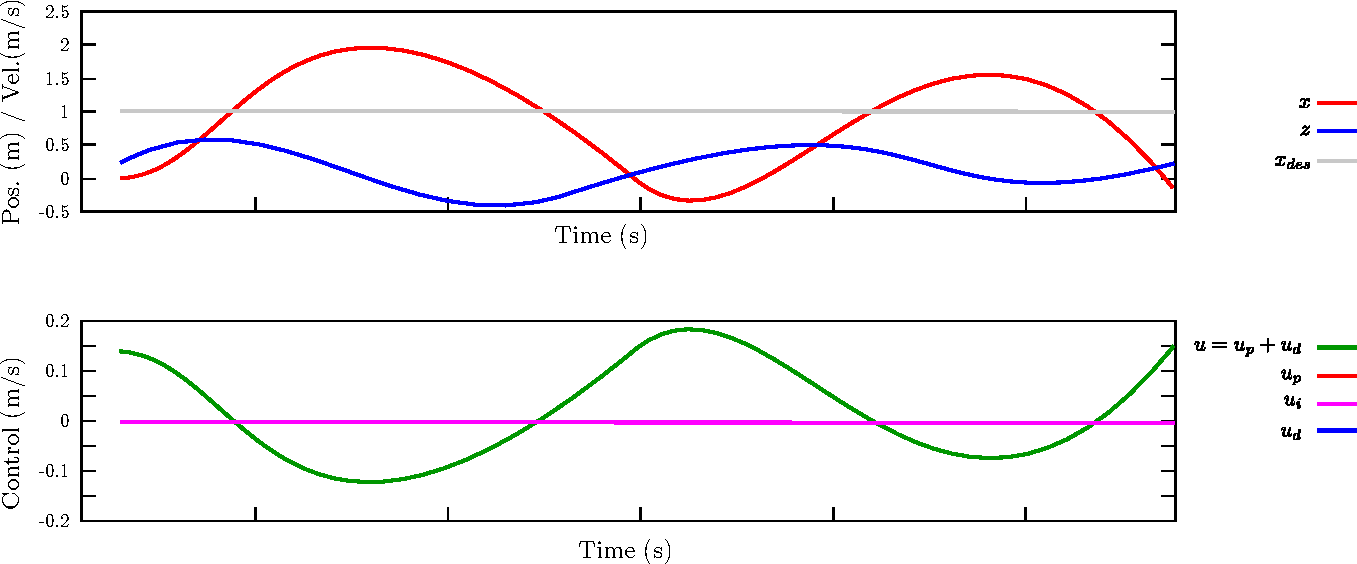
\includegraphics[width=0.8\columnwidth]{images/pid_control_position_proportional.pdf}
    \end{center}
    
\end{frame}

\begin{frame}
    \frametitle{PD-control}
    \note{Información extraída de https://youtu.be/pEVsedl2KO4?si=_cwQpRPPUnQ04B3c}
    
    \begin{itemize}
        \item PD-Control:
        \begin{equation*}
            \controlCommand_{t} = K_{d} \left( \frac{d}{d t} \error_{t} \right)
        \end{equation*}
    \end{itemize}
    
    \begin{center}
        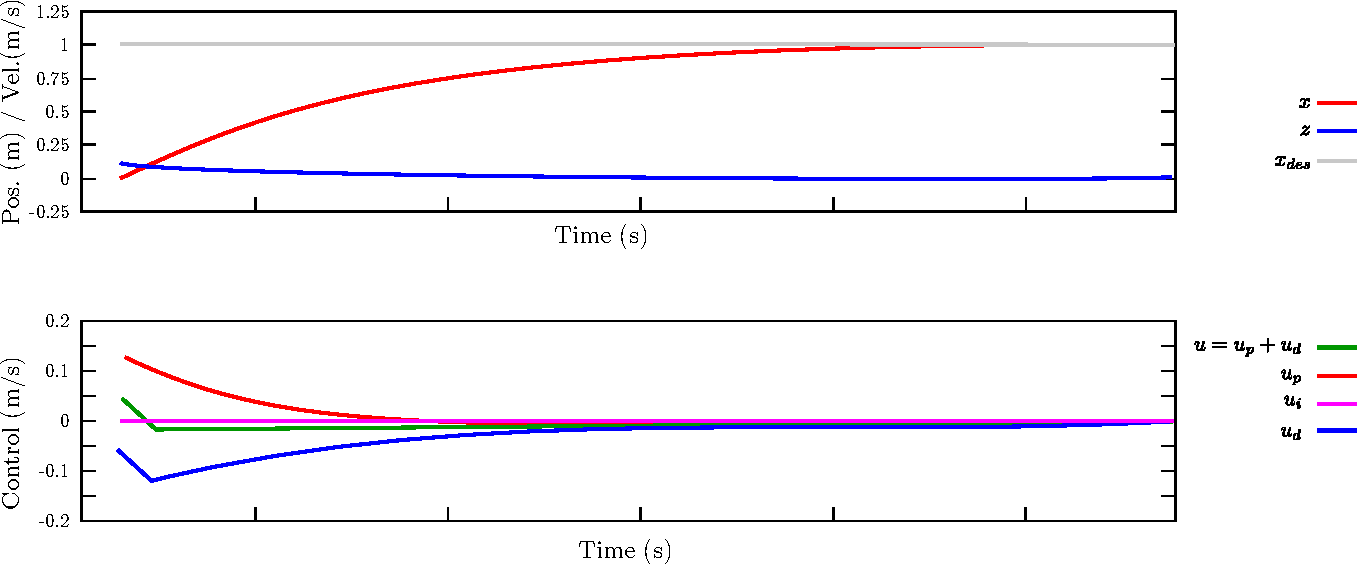
\includegraphics[width=0.8\columnwidth]{images/pid_control_position_proportional_derivative.pdf}
    \end{center}
    
\end{frame}


\begin{frame}
    \frametitle{PID-control}
    \note{Información extraída de https://youtu.be/pEVsedl2KO4?si=_cwQpRPPUnQ04B3c}
    
    \begin{itemize}
        \item PID-Control:
        \begin{equation*}
            \controlCommand_{t} = K_{p} \int_{0}^{t} \error_{t} \, dt
        \end{equation*}
    \end{itemize}
    
    \begin{center}
        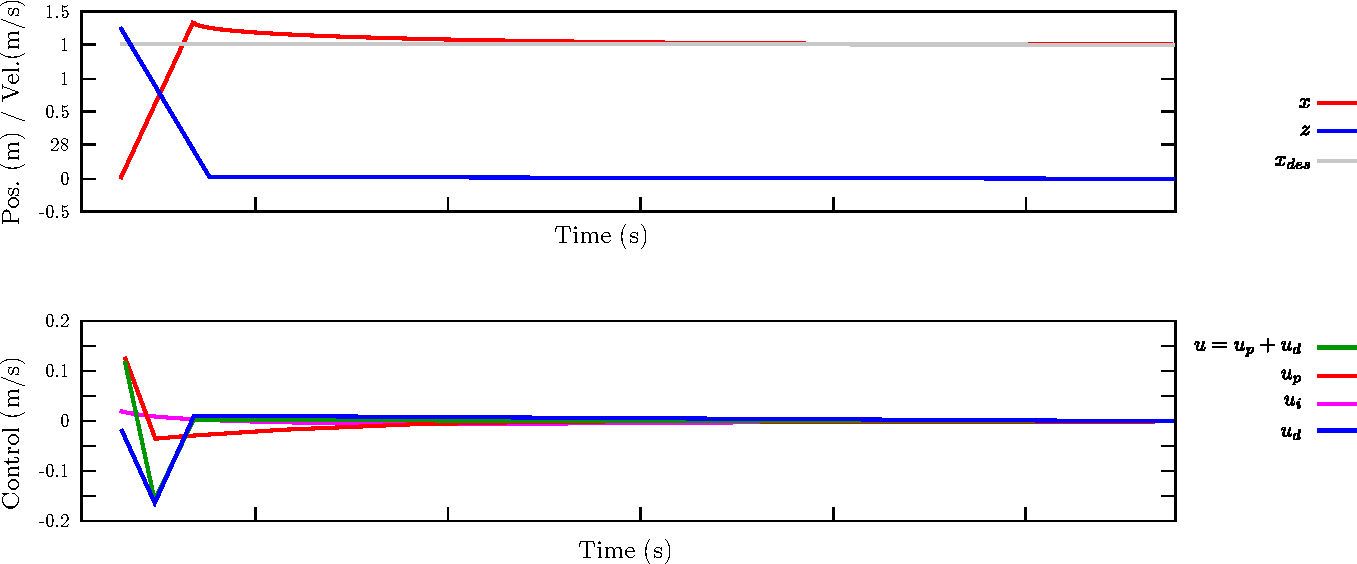
\includegraphics[width=0.8\columnwidth]{images/pid_control_position_proportional_integral_derivative.pdf}
    \end{center}
    
\end{frame}



\begin{frame}
    \frametitle{PID-control}
    \note{Información extraída de https://youtu.be/pEVsedl2KO4?si=_cwQpRPPUnQ04B3c}
    
    \begin{itemize}
        \item Estimar el error sistemático...
        \item PID-Control:
        \begin{equation*}
            \controlCommand_{t} = K_{p} \left(x_{des} - x_{t}\right) + K_{d} \left(\dot{x}_{des} - \dot{x}_{t} \right) + K_{i} \int_{0}^{t} \left( x_{des} - x_{t}\right) \, dt
        \end{equation*}
        
    \end{itemize}
    
    \begin{itemize}
        \item Funciona razonablemente para sistemas estables (con poco ruido)
        \item Puede ser peligroso en el caso en que se acumulen errores (\emph{wind-up effect})
    \end{itemize}
    
    \note{Si un robot se traba en un pozo y las ruedas siguen girando, la pose estimada por odometría y la verdadera localización del robot crece constantemente. El término integral del PID va a tomar valores enormes, ya que el error se acumula. En esta situación, si el robot se destrabara, vamos a tener una velocidad enorme y por lo tanto hacer que robot, por ejemplo, salte. Para esto el término integral puede únicamente tomar una ventana de tiempo (por ejemplo, los últimos 5 segundos).}
    
    \note{El wind-up effect se refiere a cuando le damos un comando de control al robot pero los actuadores no son capaces de alcanzar el control solicitado. Esto puede ocasionar también que se acumule error.}
    
    
    \note{Información extraída dehttps://www.zhinst.com/americas/de/resources/principles-of-pid-controllers}
    \note{Información extraída de https://newton.ex.ac.uk/teaching/CDHW/Feedback/ControlTypes.html}
    
\end{frame}

\begin{frame}
    \frametitle{PID-control: Resumen}
    \note{Información extraída de https://youtu.be/pEVsedl2KO4?si=_cwQpRPPUnQ04B3c}
    
    \begin{itemize}
        \item P = control proportional, suficiente para la mayoría de los casos
        \item PD = reduce overshoot (por ejemplo, cuando la aceleración del vehículo puede ser controlada)
        \item PI = compensa errores o bias sistemáticos
        \item PID = combinación de todas las propiedades anteriores
    \end{itemize}
    
\end{frame}
